\section{Excess velocity at arrival}

The excess velocity at arrival is the difference between the velocity of the
spacecraft at arrival and the velocity of the interloper at arrival. The
velocity of the spacecraft at arrival is denoted by $\vec{v_{\infty ,2}}$. Note
that this velocity represents the velocity after the second impulse of Lambert's
maneuver, leading to a rendezvous with the interloper. The velocity of the
interloper at arrival is $\vec{v_\text{ISO}}$. Thus, the excess velocity at
arrival is:

\begin{equation}
    \Delta v_2 = \norm{\vec{v_{\infty ,2}} - \vec{v_\text{ISO}}}
\end{equation}


\subsection{'Oumuamua}

Porkchop plots for 1I/'Oumuamua representing the excess velocity at arrival are
shown in figure \ref{fig:oumuamua-direct-prograde-transfer-porkchop-avl} and figure
\ref{fig:oumuamua-direct-retrograde-transfer-porkchop-avl}.

\begin{figure}[H]
  \centering
  \includegraphics[width=\textwidth]{static/oumuamua/direct-prograde-transfer-porkchop-avl.png}
        \caption[Direct and prograde launch energy porkchop for 'Oumuamua]{Launch energy porkchop plot for 1I/'Oumuamua for a direct and prograde
        transfer showing the isolines for
        the time of flight required for a targeting.}
  \label{fig:oumuamua-direct-prograde-transfer-porkchop-avl}
\end{figure}

\begin{figure}[H]
  \centering
  \includegraphics[width=\textwidth]{static/oumuamua/direct-retrograde-transfer-porkchop-avl.png}
        \caption[Direct and prograde launch energy porkchop for 'Oumuamua]{Launch energy porkchop plot for 1I/'Oumuamua for a direct and prograde
        transfer showing the isolines for
        the time of flight required for a targeting.}
  \label{fig:oumuamua-direct-retrograde-transfer-porkchop-avl}
\end{figure}

Again, for short times of flight, the excess velocity at arrival is higher
whereas for longer times of flight, the excess velocity at arrival is lower.
For 'Oumuamua, launches after year 2020 lead to an excess velocity at arrival of
$6 \text{ km/s}$ or greater. This is a significant amount of energy that needs to
be dissipated in order to rendezvous with 'Oumuamua.

Around later 2017, 'Oumuamua passes its periheleion. This explains the change in
the excess velocity. For dates before periohelion passage, the excess velocity
is opposite to the velocity of the interloper. After perihelion passage, the
excess velocity is aligned with the velocity of 'Oumuamua.

The only noticable difference between the prograde and retrograde transfers
appears from the $20\text{ km/s}$ excess velocity on. For retrograde transfers
with the same launch date but longer arrival dates, the excess velocity at
arrival is lower.


\subsection{Borisov}

Porkchop plots for 2I/Borisov representing the excess velocity at arrival are
shown in figure \ref{fig:borisov-direct-prograde-transfer-porkchop-avl} and figure
\ref{fig:borisov-direct-retrograde-transfer-porkchop-avl}.

\begin{figure}[H]
  \centering
  \includegraphics[width=\textwidth]{static/borisov/direct-prograde-transfer-porkchop-avl.png}
        \caption[Direct and prograde arrival excess velocity porkchop for
        Borisov]{Launch energy porkchop plot for 2I/Borisov for a direct and
        prograde transfer showing the isolines for excess velocity at arrival
        for a rendezvous.}
  \label{fig:borisov-direct-prograde-transfer-porkchop-avl}
\end{figure}

\begin{figure}[H]
  \centering
  \includegraphics[width=\textwidth]{static/borisov/direct-retrograde-transfer-porkchop-avl.png}
        \caption[Direct and retrograde arrival excess velocity porkchop for
        Borisov]{Launch energy porkchop plot for 2I/Borisov for a direct and
        retrograde transfer showing the isolines for excess velocity at arrival
        for a rendezvous.}
  \label{fig:borisov-direct-retrograde-transfer-porkchop-avl}
\end{figure}

Once again, the excess velocity at arrival for Borisov remembers the ones for
the case of 'Oumuamua. Again, the values are different and higher for the second
discovered interloper.

Similarly to 'Oumuamua, the excess velocity suffers a change in direction around
2019, when this ISO crosses its perihelion. Nevertheless, the steps between
isolines for the excess velocity at arrival are more pronounced for Borisov than
for 'Oumuamua.
